\documentclass{beamer}

\usepackage[utf8]{inputenc}
\usepackage[T1]{fontenc}
\usepackage[ngerman,shorthands=off]{babel}
\usepackage{graphicx}
\usepackage[absolute,overlay]{textpos}
\usetheme{Madrid}
\usecolortheme{seahorse} 
\setbeamertemplate{navigation symbols}{}
\usepackage[backend=biber]{biblatex}
\addbibresource{/Users/jakubmarczak/Downloads/literatur.bib}
\usepackage{csquotes}
\usepackage{hyperref}
\usepackage{wasysym}
\usepackage{xcolor}

\title{Abschlussprojekt}
\author{Sergio Alvarez, Ilkay Aydin, Jakub Marczak, Nermine Msolly}
\date{\today}

\begin{document}

% Folie 1
\frame{\titlepage}

% Folie 2
\begin{frame}
    \frametitle{Untersuchungsziele}
    \begin{enumerate}
        \item Population verstehen
        \item Nierenschädigung durch Vancomycin
        \item[$\rightarrow$] Verhalten von SCr- und eGFR-Werten
        \item[$\rightarrow$] Auswirkung vom Vancomycin-Spiegel auf Nierenmarker
        \item Mortalitätsanalyse
        \item[$\rightarrow$] Einfluss des Schweregrades der Erkrankung auf die Mortalität
        \item[$\rightarrow$] Welche Einflüsse begleiten die Mortalität am meisten?
        \item {\color{black!55} Anhang}
    \end{enumerate}
\end{frame}

% Folie 3
\begin{frame}
    \frametitle{Population verstehen}
    \begin{figure}
        \centering
        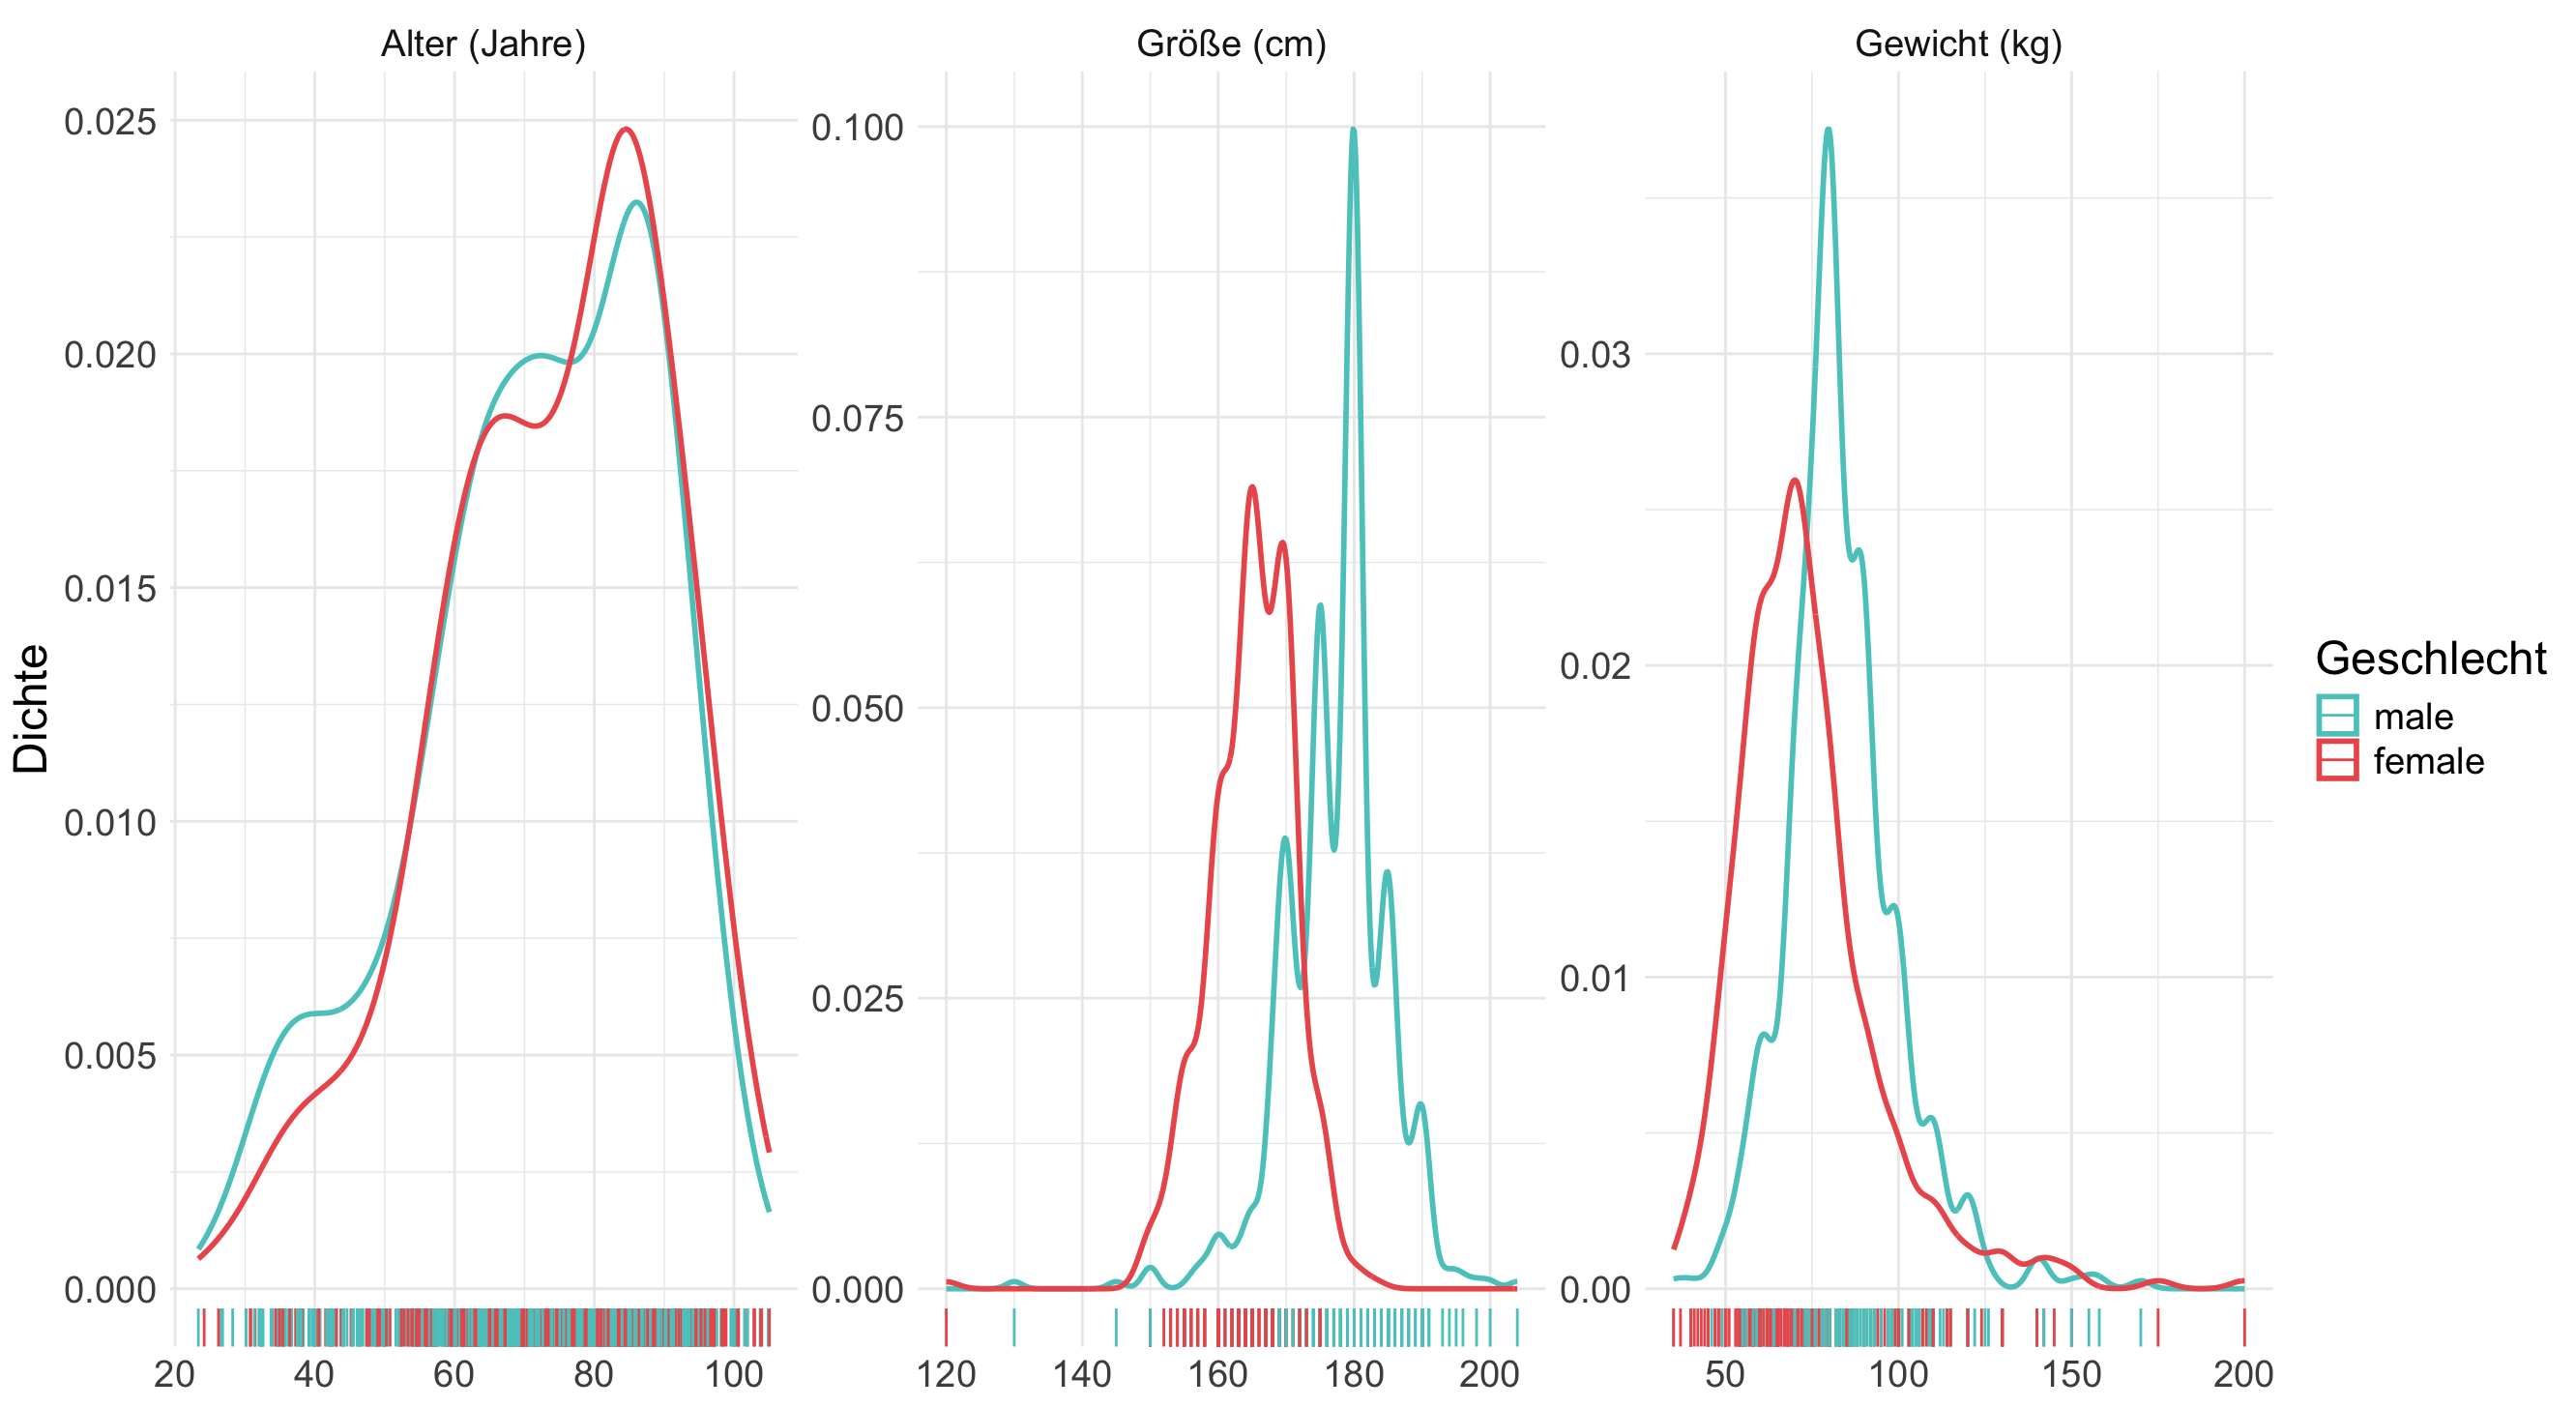
\includegraphics[width=1\linewidth]{population.png}
        \caption{Kerndichteschätzungen mit Gaußkern für Alter, Größe und Gewicht.}
    \end{figure}
\end{frame}

% Folie 4
\begin{frame}
    \frametitle{Verhalten von SCr- und eGFR-Werten}
    \begin{figure}
        \centering
        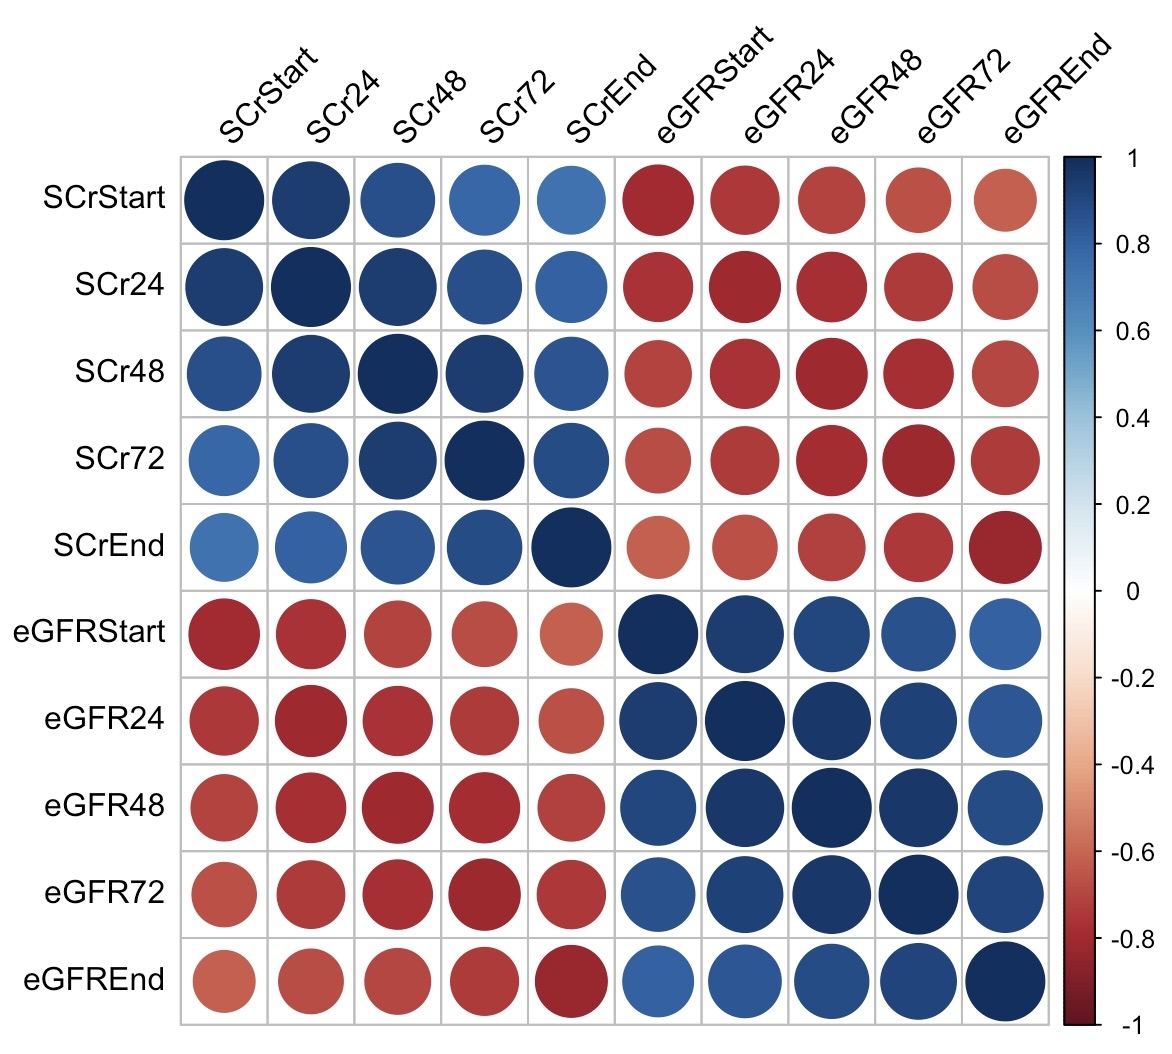
\includegraphics[width=0.6\linewidth]{corrplot nierenmarker.jpeg}
        \caption{Korrelationsplot zwischen SCr- und eGFR-Werten als Nierenmarker.}
    \end{figure}
\end{frame}

% Folie 5
\begin{frame}
    \frametitle{Auswirkung vom Vancomycin-Spiegel auf Nierenmarker}
    \begin{figure}
        \centering
        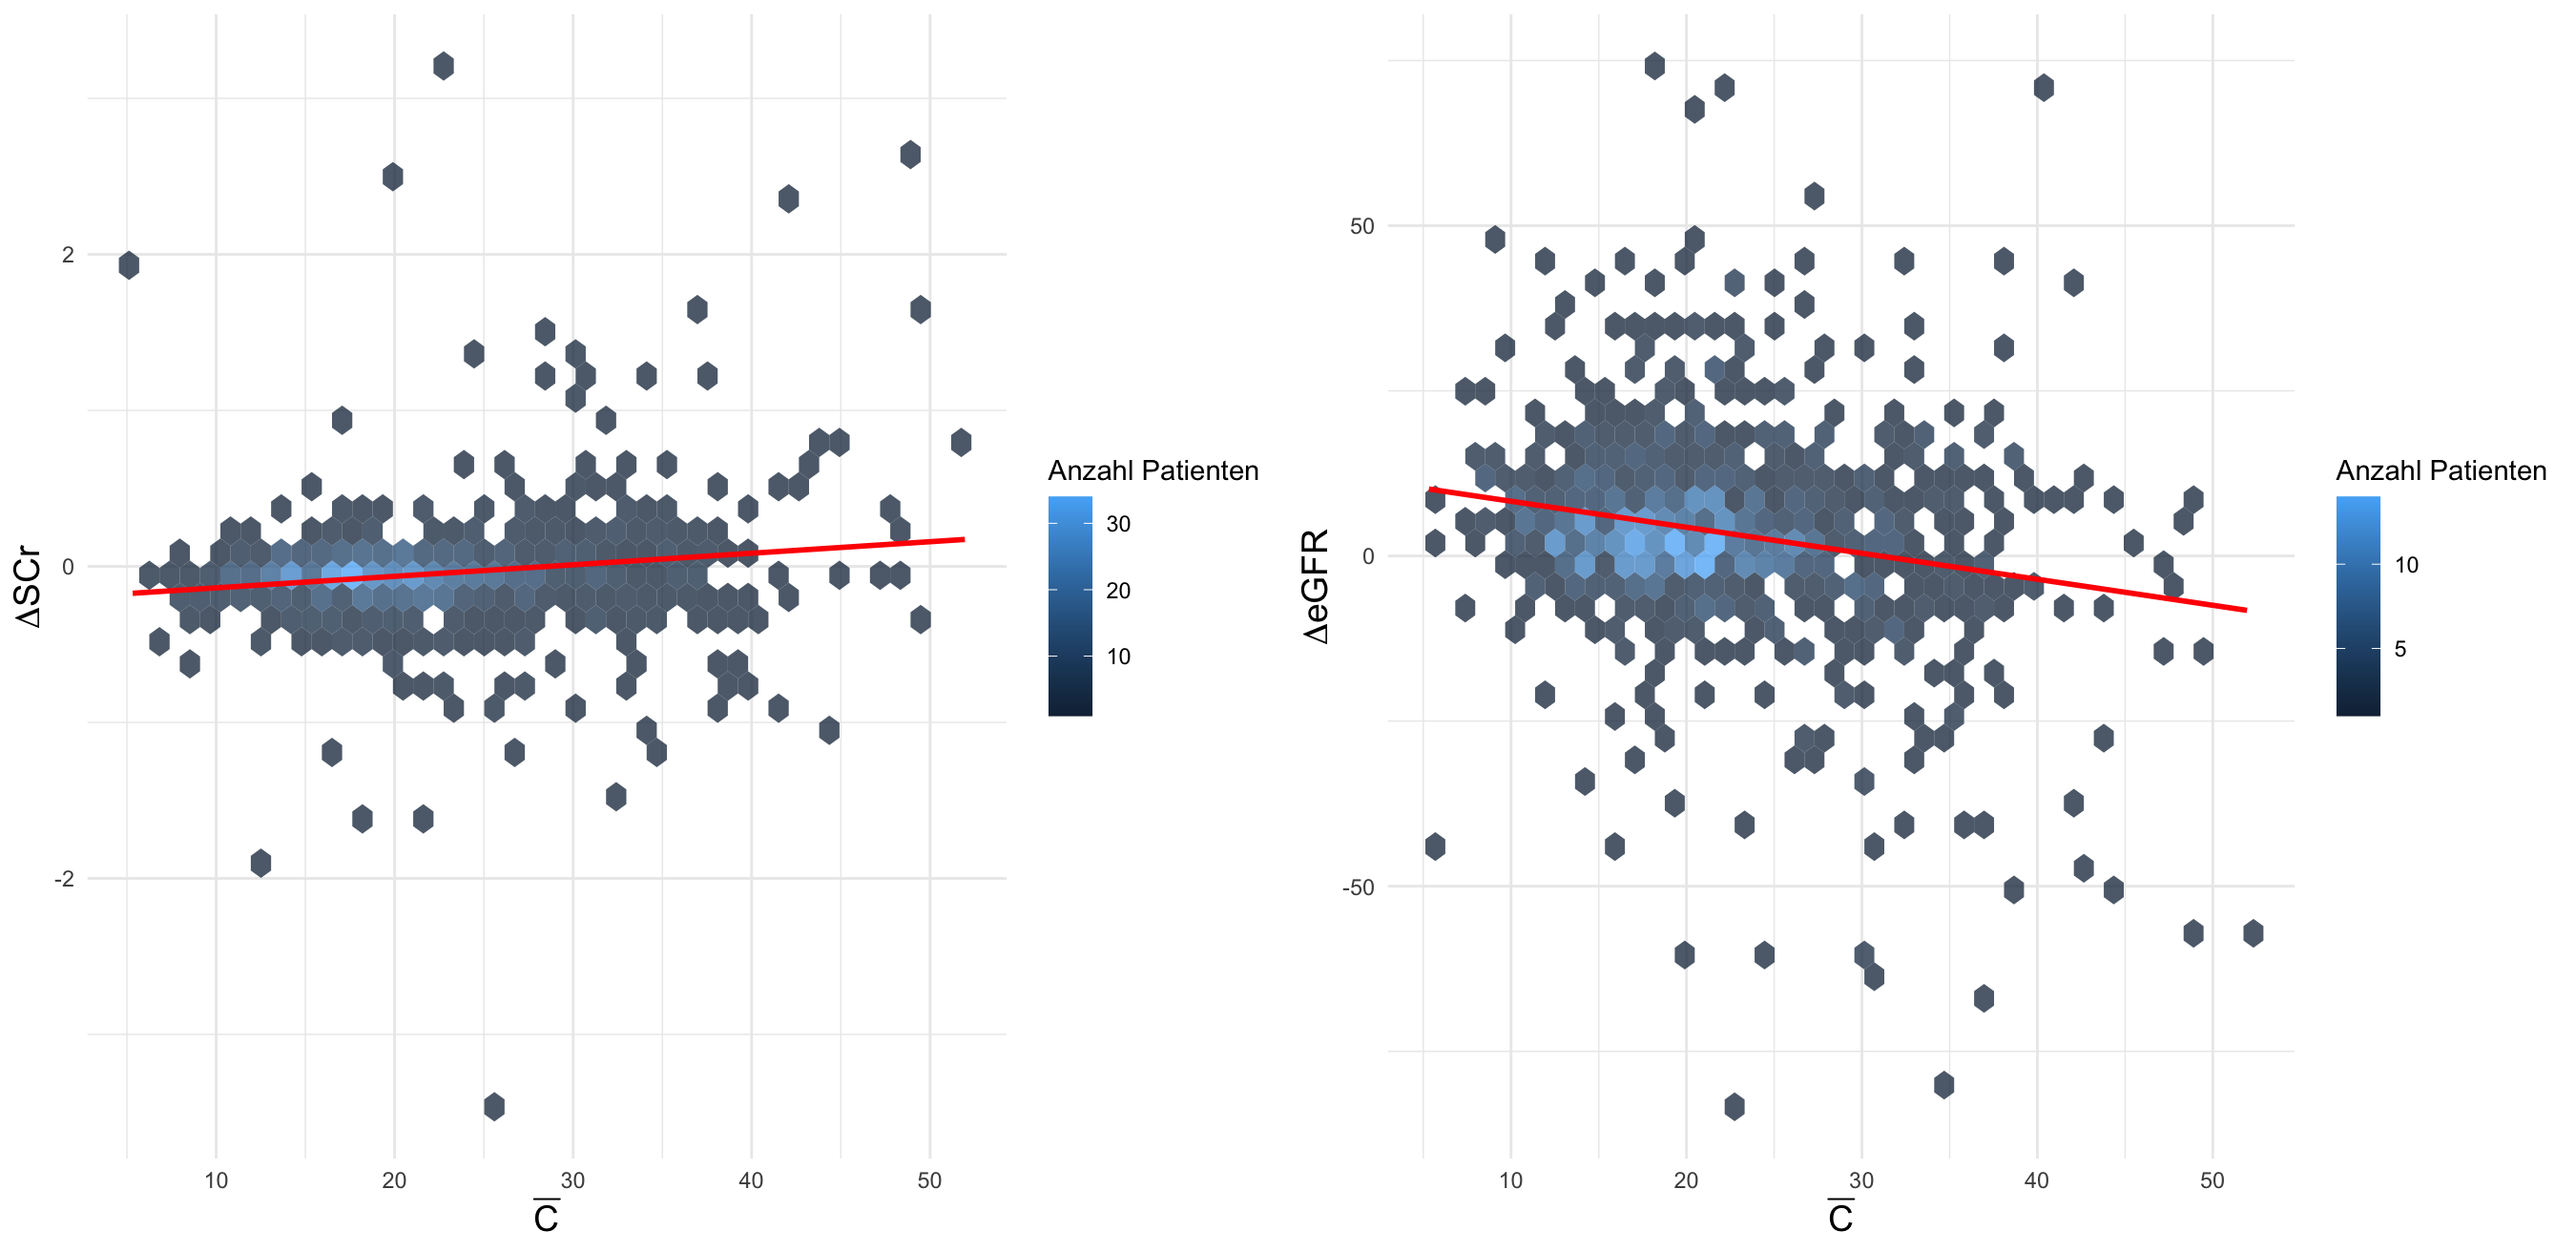
\includegraphics[width=1\linewidth]{ZhSCreGFR.png}
        \caption{Hexbin-Plots von SCr und eGFR in Abhängigkeit von der mittleren C-Konzentration ($\bar{C}$).}
    \end{figure}
\end{frame}

% Folie 6
\begin{frame}
    \frametitle{Auswirkung vom Vancomycin-Spiegel auf Nierenmarker}
    \begin{figure}
        \centering
        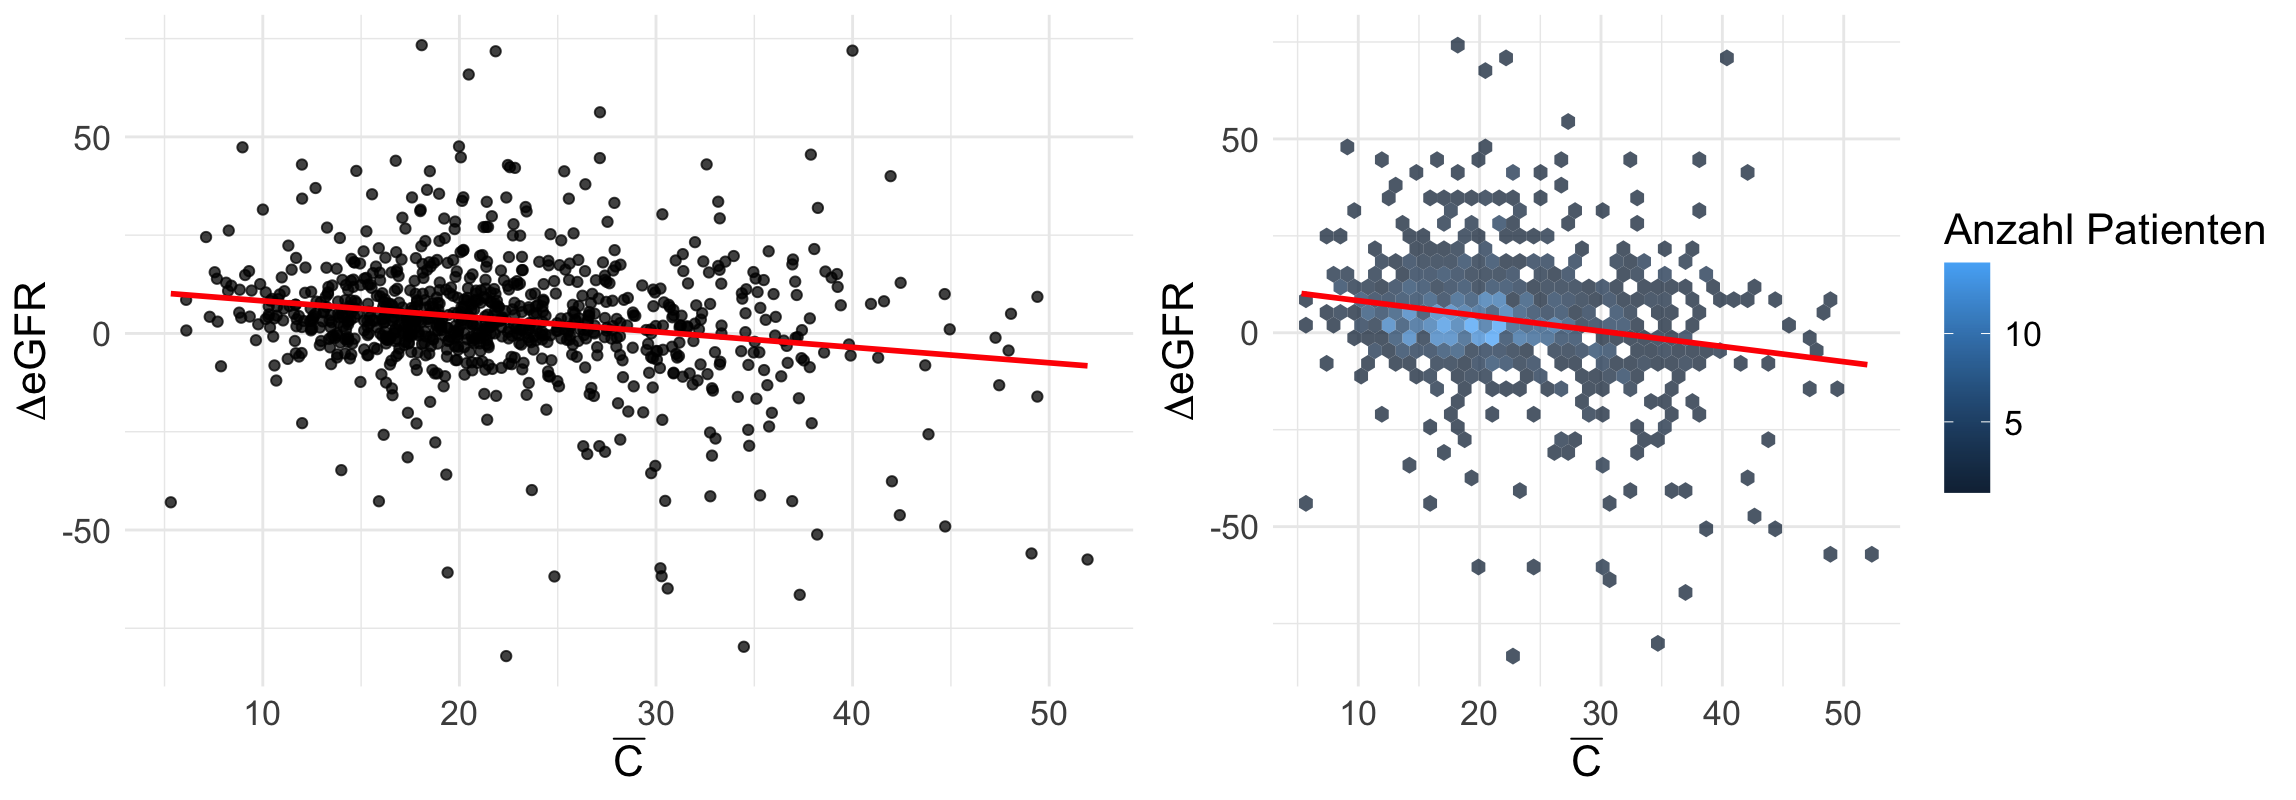
\includegraphics[width=1\linewidth]{HexScat.png}
        \caption{Vergleich der Darstellung desselben Datensatzes als Scatterplot und Hexbin-Plot.}
    \end{figure}
\end{frame}

% Folie 7
\begin{frame}
    \frametitle{Einfluss des Schweregrades der Erkrankung auf die Mortalität}
    \begin{figure}
        \centering
        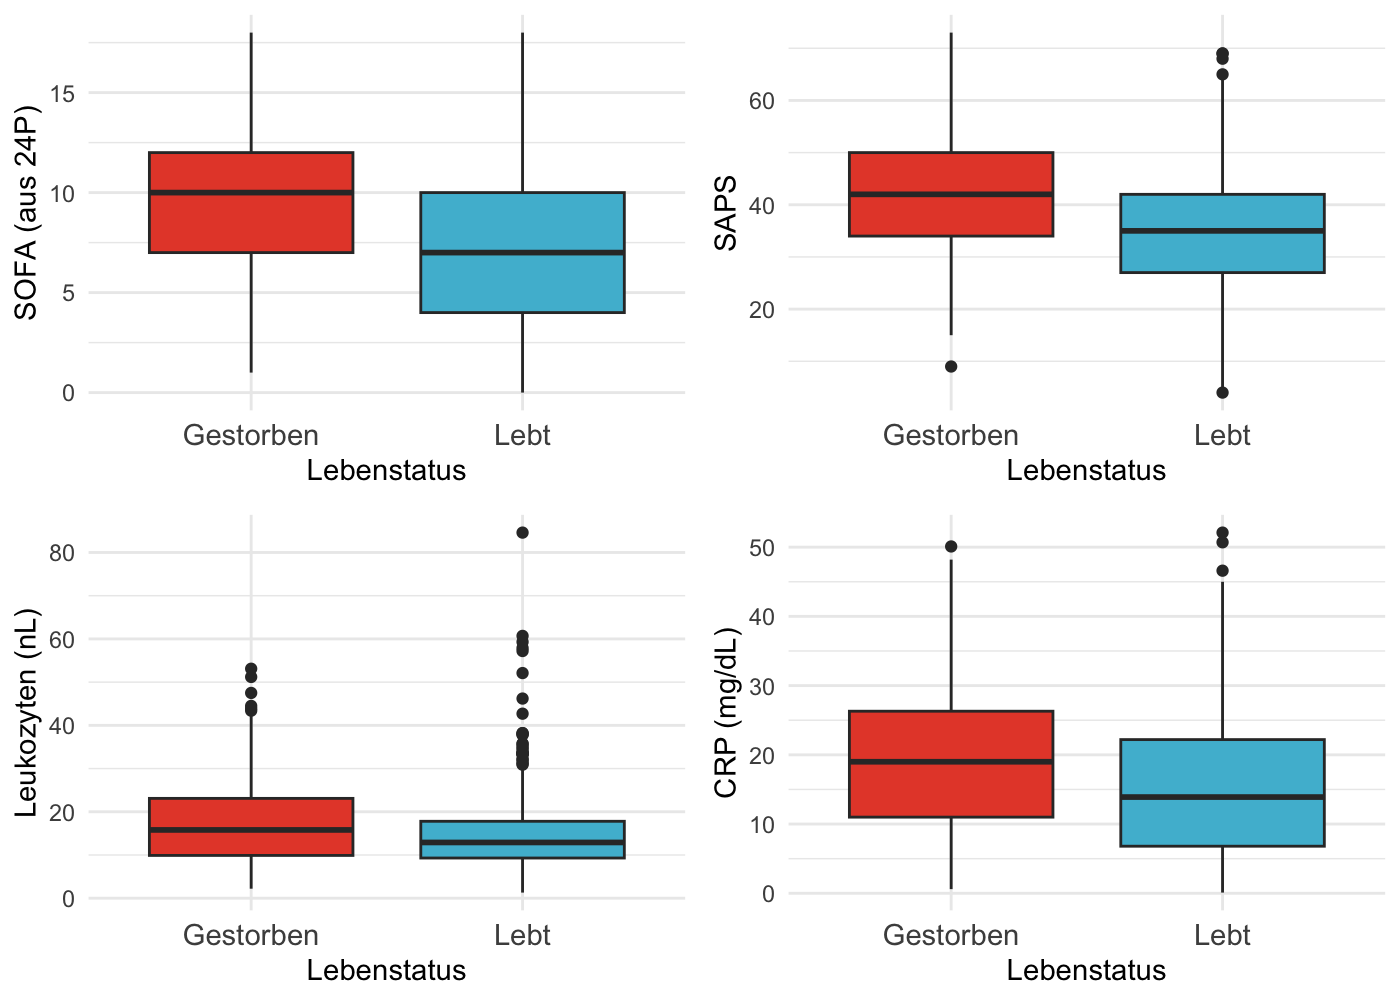
\includegraphics[width=0.7\linewidth]{Boxplot Lebenstatus.png}
        \caption{Boxplots der Schweregradvariablen zu Therapiebeginn (erste 24h), gruppiert nach Mortalitätsstatus (lebt vs. gestorben).}
    \end{figure}
\end{frame}

% Folie 8
\begin{frame}
    \frametitle{Welche Komorbiditäten begleiten die Mortalität am meisten?}
    \begin{figure}
        \centering
        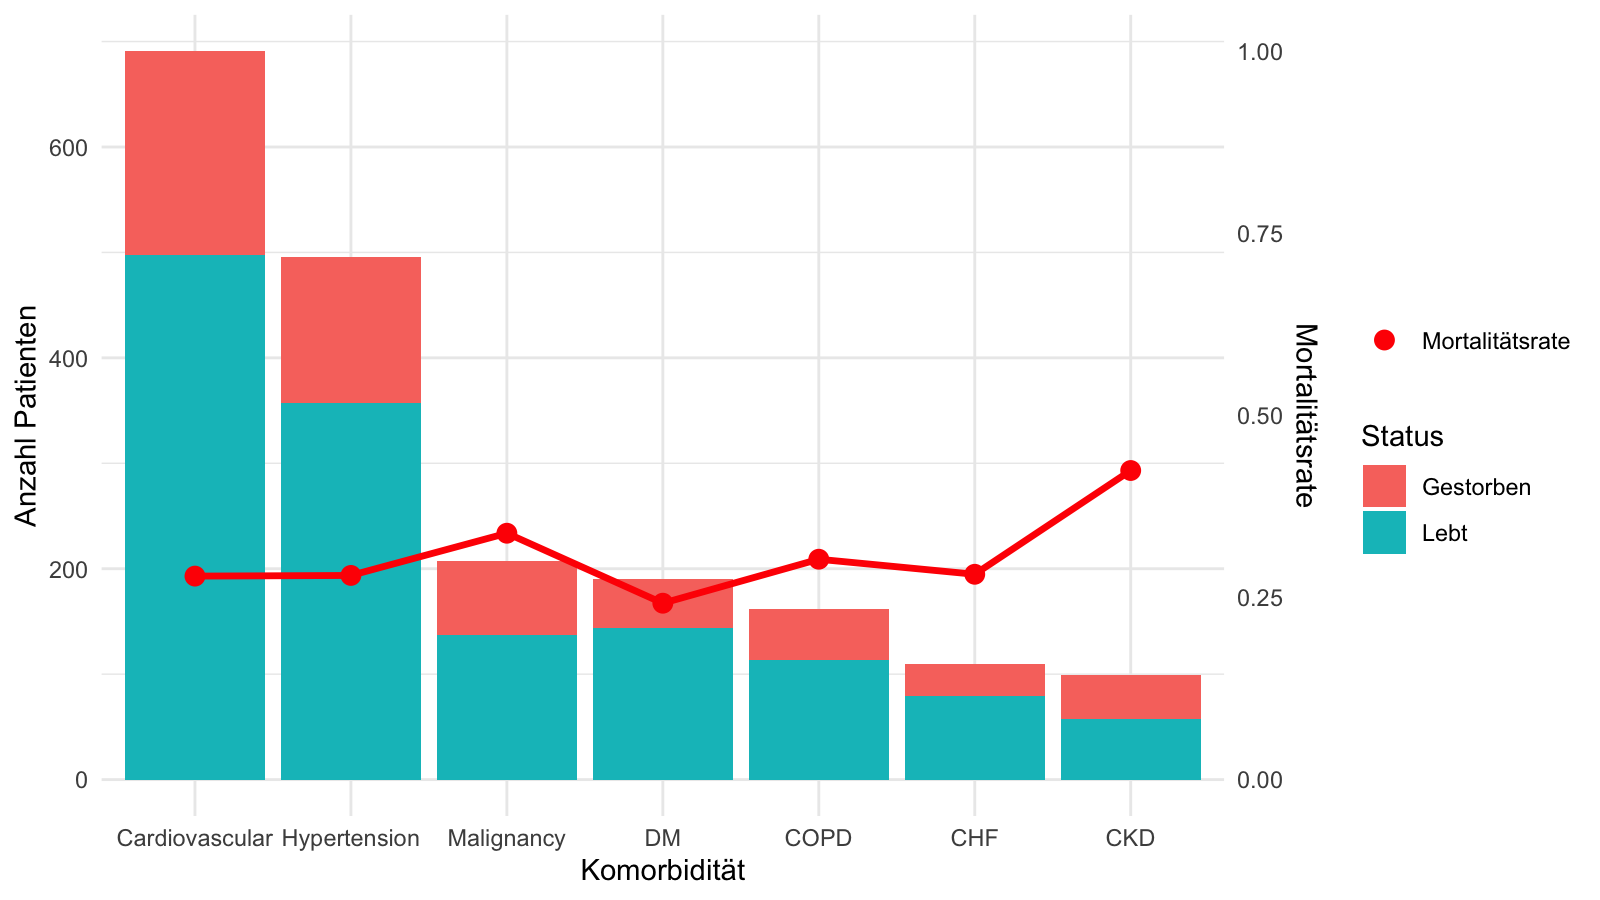
\includegraphics[width=1\linewidth]{Komor x Mort.png}
        \caption{Barplot Anzahl von Patienten und Mortalitätsrate abhängig von Komorbiditäten.}
    \end{figure}
\end{frame}

% Folie 9
\begin{frame}
    \frametitle{Welche Nephrotoxine begleiten die Mortalität am meisten?}
    \begin{figure}
        \centering
        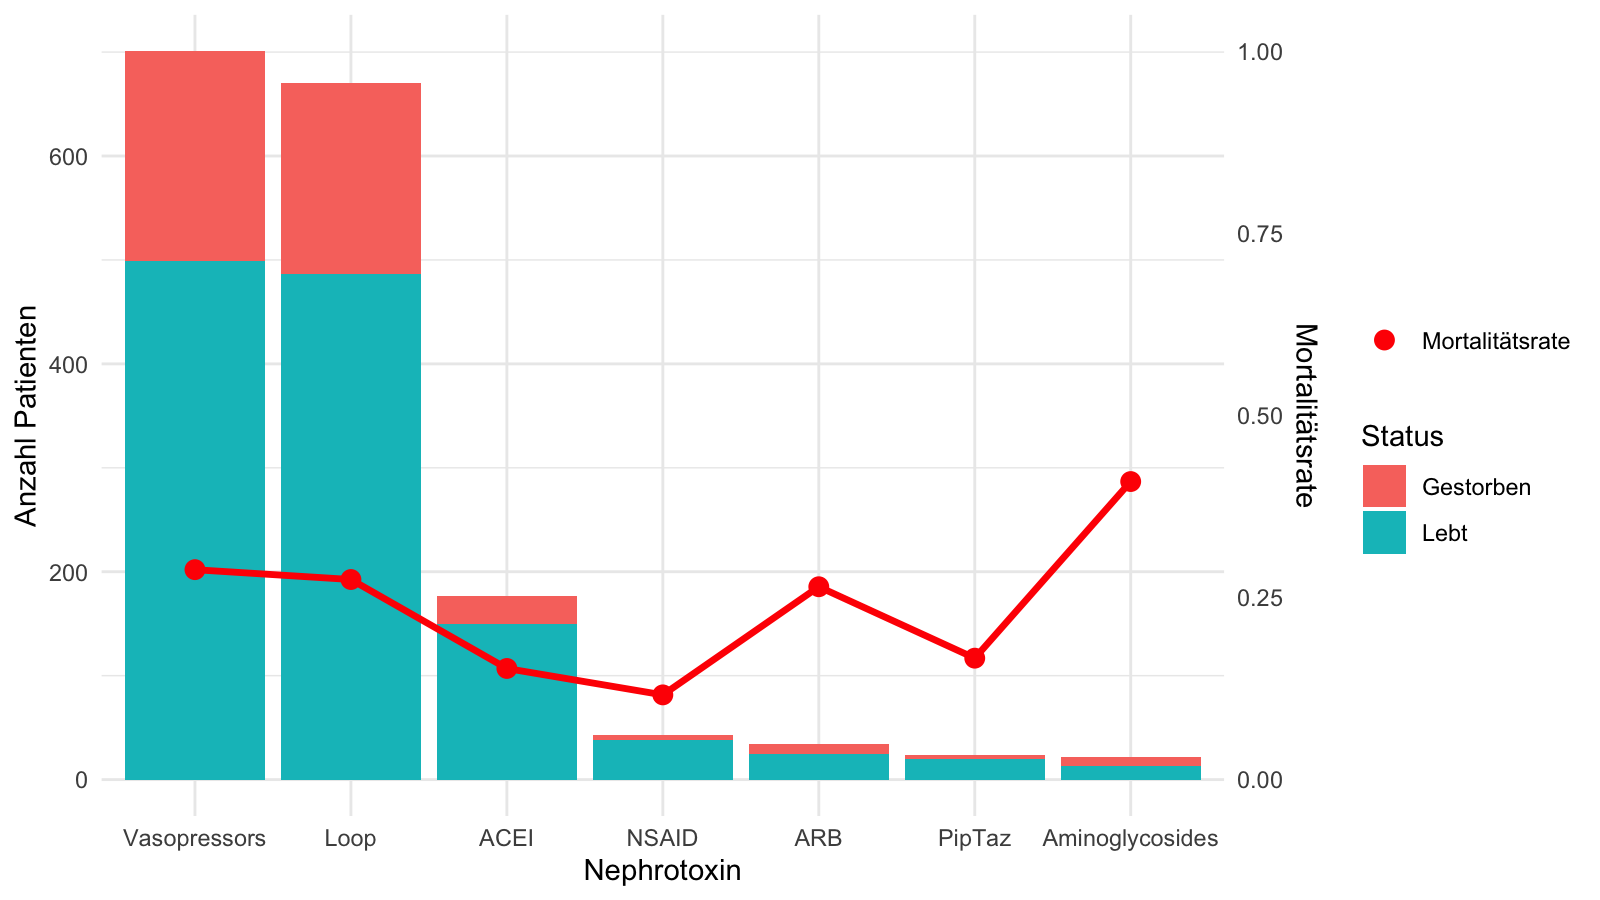
\includegraphics[width=1\linewidth]{Nephro x Mort 2.png}
        \caption{Barplot Anzahl von Patienten und Mortalitätsrate abhängig von Nephrotoxinen.}
    \end{figure}
\end{frame}

% Folie 10 - NERMINE
\begin{frame}
    \frametitle{Therapiedauer nach Mortalitätsstatus}
    \begin{figure}
        \centering
        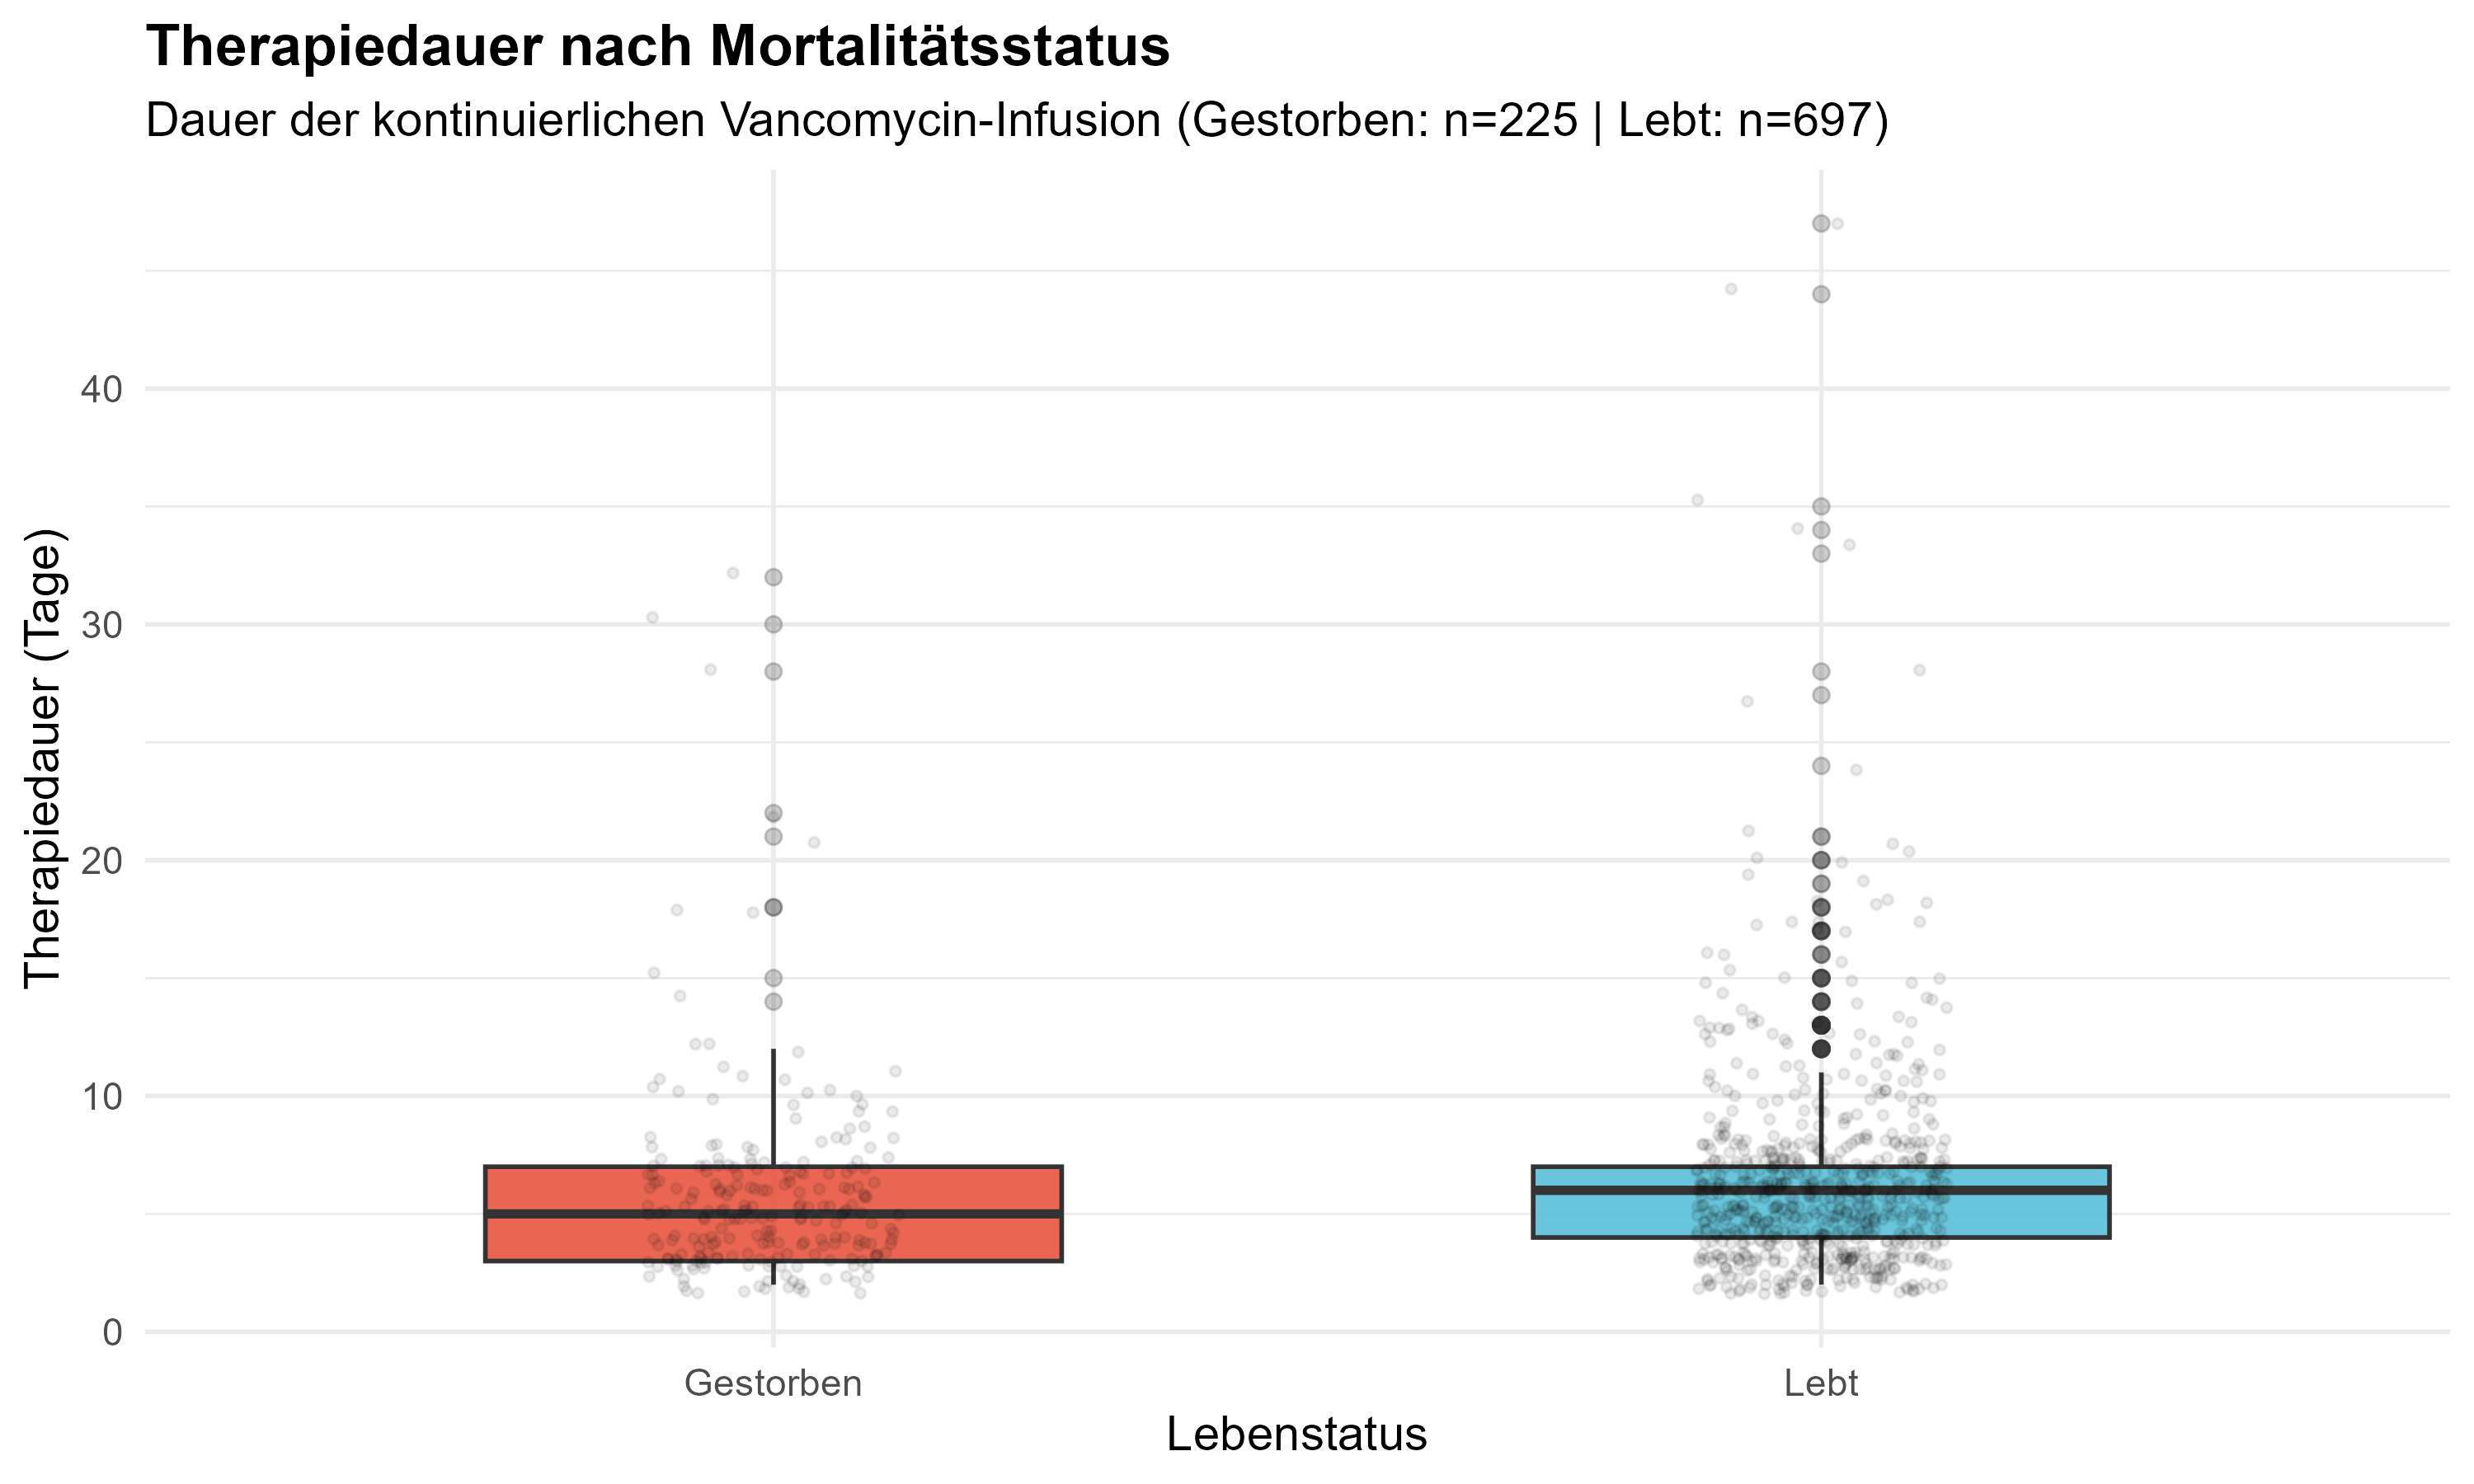
\includegraphics[width=0.85\linewidth]{therapiedauer_mortalitaet.png}
        \caption{Dauer der Vancomycin-Therapie nach Mortalitätsstatus.}
    \end{figure}
\end{frame}

% Folie 11 - NERMINE
\begin{frame}
    \frametitle{Mortalitätsrate nach C24-Quartilen}
    \begin{figure}
        \centering
        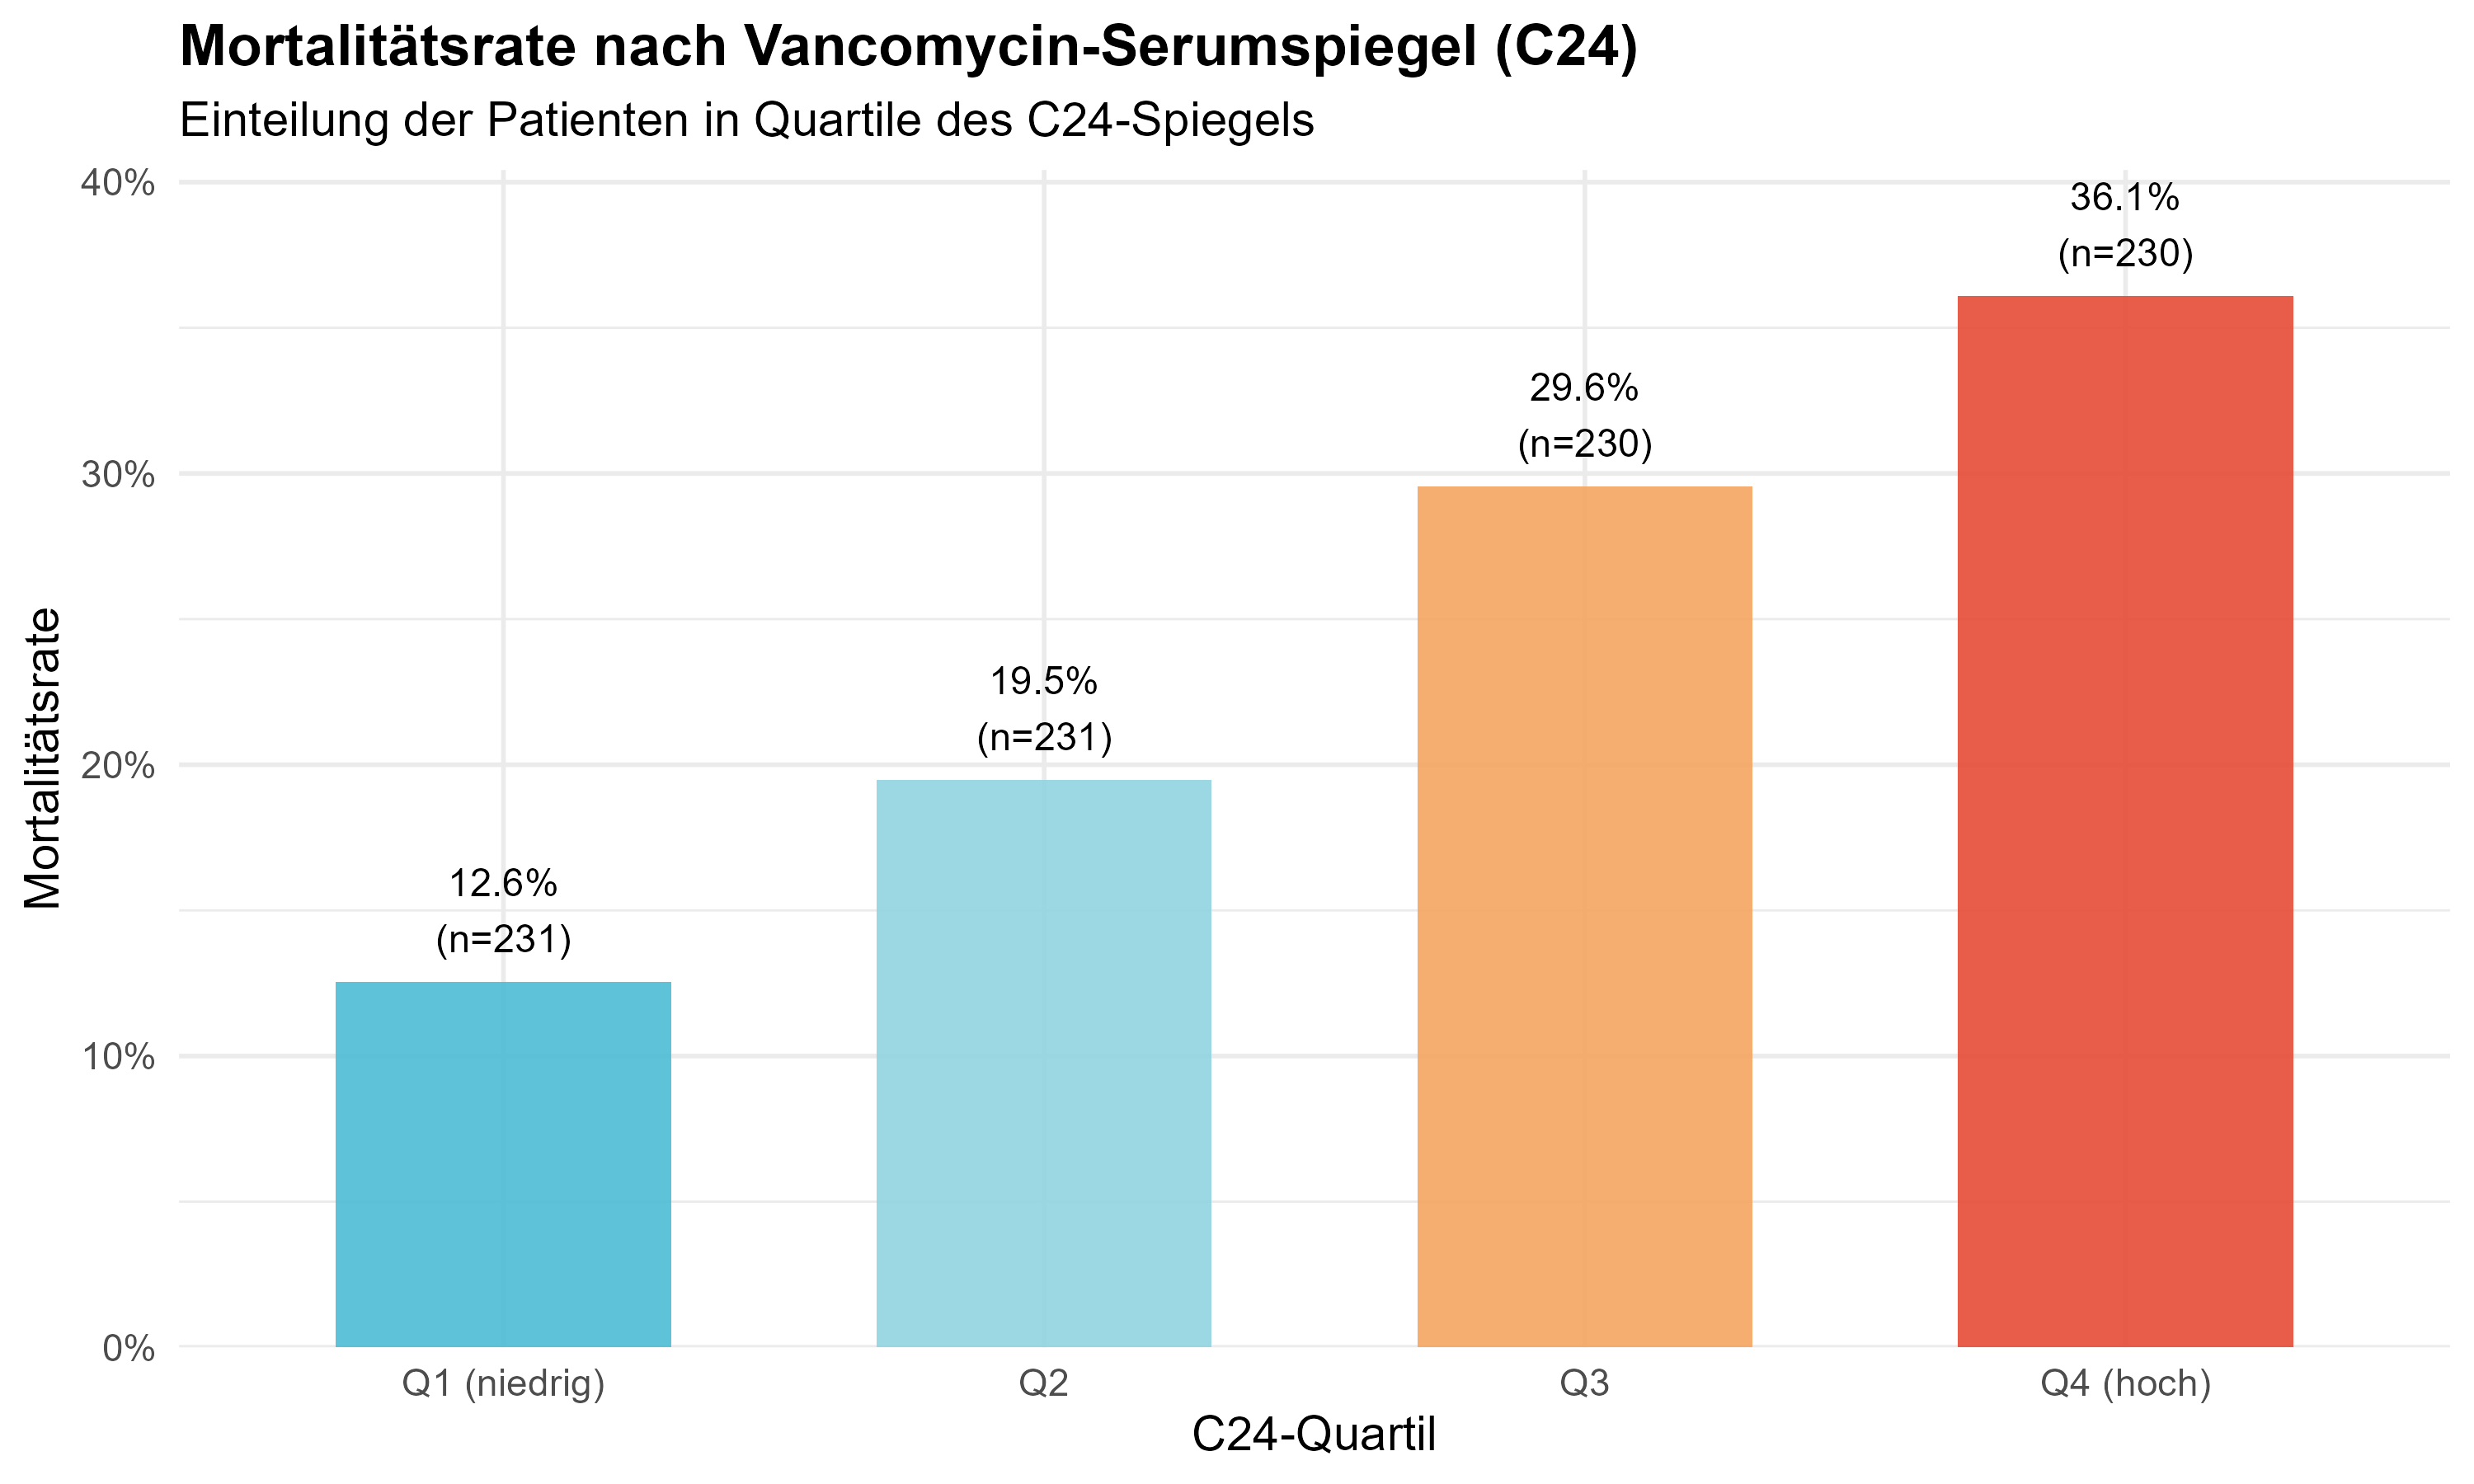
\includegraphics[width=0.85\linewidth]{mortalitaetsrate_c24_quartile.png}
        \caption{Mortalitätsrate nach Quartilen des Vancomycin-Serumspiegels (C24).}
    \end{figure}
\end{frame}

% Folie 12
\begin{frame}
    \frametitle{Zusammenfassung}
\end{frame}

% Folie 13
\begin{frame}
    \frametitle{Anhang}
    \begin{itemize}
        \item Genutzte R-Pakete
        \begin{itemize}
            \item ggplot2
            \item gridExtra
            \item tidyr
            \item dplyr
            \item corrplot
            \item scales
            \item hexbin
        \end{itemize}
    \end{itemize}
\end{frame}

\end{document}
